
\section{Глава 4. Проектирование системы для отправки сообщений на борт дрона с наземной станции}

Отправка видеопотока производится за счет UDP пакетов.  Данный протокол не гарантирует доставку сообщений, но позволяет уменьшить задержку получения потока, что более критично. Проверены кодеки jpeg, h264, omxh264enc, из них самым стабильным по задержке оказался h264. Задержка составила 150 мс.

После включения дрона и загрузки ОС RPi производится удаленное подключение к Raspberry Pi.
Запускается gstreamer для передачи изображения с rpicamsrc на адрес наземной станции UDP пакетами. На наземной станции запускается gstreamer для их получения. Команды представлены на листинге \ref{lst:12}:
\begin{Program}[H]
	\caption{Измененные параметры в launch файле mavros} \label{lst:12}
\begin{MyCode}
# На наземной станции запускается:
$ gst-launch-1.0 udpsrc port=5000 ! gdpdepay !\
rtph264depay ! avdec_h264 ! videoconvert !\
autovideosink sync=false
	
# На Raspberry Pi:
$ gst-launch-1.0 rpicamsrc bitrate=1000000 !\
'video/x-h264,width=640,height=480' ! h264parse !\
queue ! rtph264pay config-interval=1 pt=96 ! gdppay !\
udpsink host=[IP ПК] port=5000
	
\end{MyCode}
\end{Program}
\begin{MyCode}
	На ПК запускается:
	\$ gst-launch-1.0 udpsrc port=5000 ! gdpdepay ! rtph264depay ! avdec_h264 ! videoconvert ! autovideosink sync=false
	
	На Raspberry:
	\$ gst-launch-1.0 rpicamsrc bitrate=1000000 ! 'video/x-h264,width=640,height=480' ! h264parse ! queue ! rtph264pay config-interval=1 pt=96 ! gdppay ! udpsink host=[IP ПК] port=5000
	%\$ gst-launch-1.0 -v rpicamsrc bitrate=10000000 rotation=180 exposure-mode=10 awb-mode=0 awb-gain-red=1 awb-gain-blue=2 iso=800 shutter-speed=10000 contrast=50 ! "image/jpeg,width=640,height=480,framerate=30/1" ! udpsink host=192.168.1.148 port=9000
	
\end{MyCode}
%https://www.raspberrypi.org/forums/viewtopic.php?t=196176

%https://docs.opencv.org/master/db/da9/tutorial_aruco_board_detection.html
%https://diydrones.com/group/voltarobots/forum/connect-telemetry-through-tcp-udp?commentId=7447824%3AComment%3A1590641
%https://stackoverflow.com/questions/7669240/webcam-streaming-using-gstreamer-over-udp

%Для использования аппаратного кодирования:
%\begin{MyCode}
%PC(autovideosink sync=false not needed for gscam):
%gst-launch-1.0 udpsrc port=5000 ! gdpdepay ! rtph264depay ! avdec\_h264 ! videoconvert ! autovideosink sync=false

%RPI stream:

%gst-launch-1.0 rpicamsrc bitrate=1000000 ! "video/x-raw,width=640,height=480,framerate=30/1" ! omxh264enc target-bitrate=1000000 control-rate=variable ! 'video/x-h264,width=640,height=480'! h264parse ! queue ! rtph264pay config-interval=1 pt=96 ! gdppay ! udpsink host=192.168.1.253 port=5000
%\end{MyCode}

tab-1 (запуск нод gscam и aruco\_gridboard по полученному топику): 
export GSCAM\_CONFIG="udpsrc port=5000 ! gdpdepay ! rtph264depay ! avdec\_h264 ! videoconvert"
roslaunch aruco\_gridboard detection\_rpicam.launch

tab-2 (запуск окружения маврос): roslaunch mavros apm.launch

tab-3 (The messages SET\_GPS\_GLOBAL\_ORIGIN and a SET\_HOME\_POSITION are sent with a script before starting to use the system.): rosrun aruco\_gridboard set\_origin.py

tab-4 (запуск rviz на усмотрение): rosrun rviz rviz -d catkin\_ws/src/aruco\_gridboard/data/aruco\_grid.rviz

запуск rpi
gst-launch-1.0 rpicamsrc bitrate=1000000 ! 'video/x-h264,width=640,height=480' ! h264parse ! queue ! rtph264pay config-interval=1 pt=96 ! gdppay ! udpsink host=192.168.1.53 port=5000

для задержки в 80мс на пк:\\
clever@clever-dev: gst-launch-1.0 udpsrc port=5000 ! "image/jpeg,width=640,height=480,framerate=30/1" ! jpegdec ! videoconvert ! autovideosink sync=false

на рпи:
gst-launch-1.0 rpicamsrc bitrate=10000000 iso=800 shutter-speed=10000 contrast=50 ! "image/jpeg,width=640,height=480,framerate=30/1" ! udpsink host=192.168.1.53 port=5000

export GSCAM\_CONFIG="udpsrc port=5000 ! "image/jpeg,width=640,height=480,framerate=30/1" ! jpegdec ! videoconvert"
\$ rostopic echo /mavros/vision\_pose/pose

-----
Собрали через каткин драйвер gscam, запустили roscore, осталось изменить лаунч и получить поток.
Для создания топиков необхходимо настроить маврос.

В /opt/ros/melodic/share/mavros/launch/apm.launch меняется параметр fcu\_url для общения с телеметрией по порту полетника с помощью ser2net proxy:
<arg name="fcu\_url" default="tcp://192.168.10.16:2000" />
% ~\ref{fig:px4}
\begin{figure}[H]
	\centering
	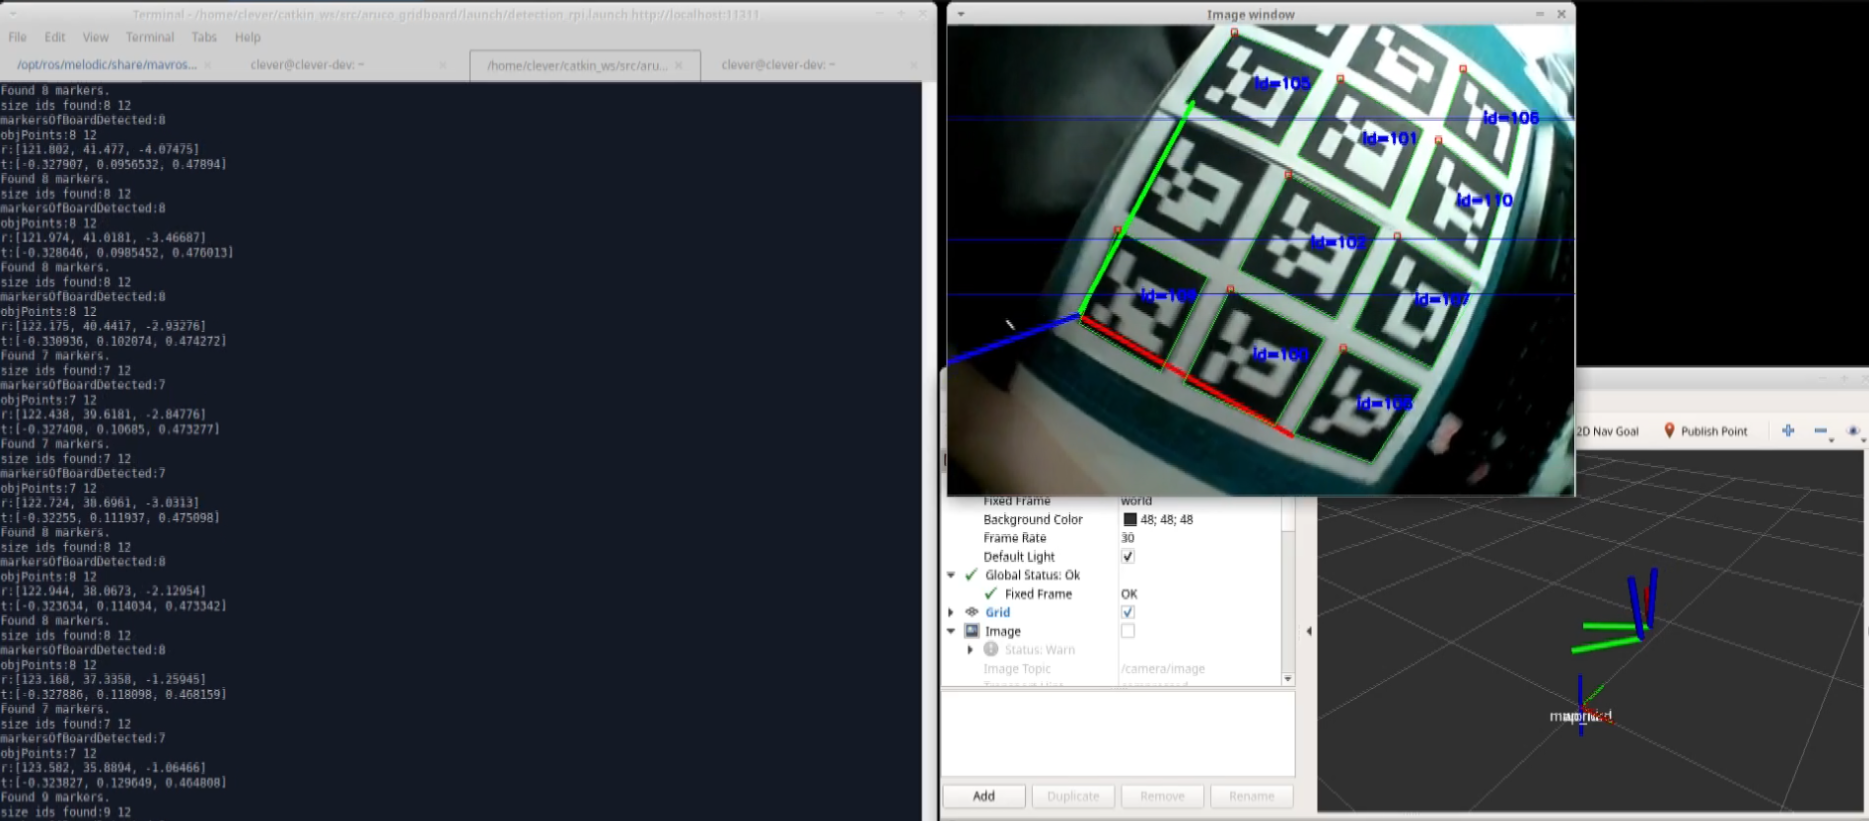
\includegraphics[width=0.9\linewidth]{pics/px4}
	\caption{ GStreamer pads (sink, src\_0, src\_1)
	}
	\label{fig:px4}
\end{figure}
